\documentclass[12pt,a4paper,svgnames]{article}
\usepackage{amsmath}
\usepackage{fullpage}
\usepackage{amsfonts}
\usepackage{amssymb,amsthm}
\usepackage{makeidx}
\usepackage{graphicx}
\usepackage{float}
\usepackage{wrapfig}
\usepackage{algorithm}
\usepackage{algorithmicx}
\usepackage{ccaption}
\usepackage{xspace}
\usepackage{stmaryrd}
\usepackage{mathtools}
\usepackage{algpseudocode}
\usepackage{titlesec}
\usepackage{pifont}

%\usepackage{floatrow}
\usepackage{tikz}
\usetikzlibrary{automata,trees,fit,backgrounds,shapes,snakes}
\usetikzlibrary{decorations.shapes}
\usepackage{float}
\usepackage{array}


\usepackage{xcolor}
\titleformat*{\section}{\bfseries}
\usepackage{leestd}
\usepackage{enumitem}
\author{Lee Gao (lg342)}
\title{ENGRI 1101 Problem Set 9}
\begin{document}
\maketitle


\begin{enumerate}[label=\textbf{Exercise \arabic*\ }]
\item Consider the small Sudoku puzzle given below. For those not familiar, the object of Sudoku is to
fill in the empty cells with the numbers 1 through 4, such that no number appears twice in any row,
column, or bold $2 \times 2$ block. Give an integer program whose solution you could use to find the answer
to this puzzle. Note that with minimal modification, your integer program should be able to solve
any $4 \times 4$ Sudoku puzzle. Hence solving this puzzle by hand and then constraining each variable to
correspond to that solution is not an acceptable answer. (Hint: you should use 64 decision variables,
each constrained to be 0 or 1, where setting $x_{ijk} = 1$ corresponds to setting the cell in the $i^{\text{th}}$ row and
the $j^{\text{th}}$ column to take value $k$)
\begin{figure}[H]
\centering
\renewcommand{\arraystretch}{1.3}
\caption{Sudoku Instance}
\begin{tabular}{!{\vrule width 2pt}c|c!{\vrule width 2pt}c|c!{\vrule width 2pt}}
\noalign{\hrule height 2pt}
& 2 & 1 & \\ \hline
& & & 2 \\ \noalign{\hrule height 2pt}
& 4 &  & \\ \hline
3 & & &  \\ \noalign{\hrule height 2pt}
\end{tabular}
\end{figure}

\vspace{4mm}
As discussed in the problem statement, let $x_{ijk} = 1$ denote whether the $(i,j)$ cell is filled with $k$. Let $\g{dom} = \Rec{1,2,3,4}$ We would like to consider the following constraints:
\begin{dingautolist}{192}
\item Every cell has exactly one value 
$$
\forall i,j \in \g{dom}. \sum_{k\in \g{dom}} x_{ijk} = 1
$$
\item Every column has only one cell containing $k$
$$
\forall k,j \in \g{dom}. \sum_{i \in \g{dom}} x_{ijk} = 1
$$
\item Likewise for rows
$$
\forall k,i \in \g{dom}. \sum_{j \in \g{dom}} x_{ijk} = 1
$$
\item That each submatrix has only one cell containing $k$.
We will partition the matrix into the blocks
$$
\mat{X_1 & X_2 \\ X_3 & X_4}
$$
so that we can let
\begin{align*}
B_1 &= \Rec{(1,1),(1,2),(2,1),(2,2)} \\
B_2 &= \Rec{(1,3),(1,4),(2,3),(2,4)} \\
B_3 &= \Rec{(3,1),(3,2),(4,1),(4,2)} \\
B_4 &= \Rec{(3,3),(3,4),(4,3),(4,4)}
\end{align*}
and we can impose the constraint that
$$
\forall m,k \in \g{dom}. \sum_{(i,j) \in B_m} x_{ijk} = 1
$$
\item The given cells. Here, we will let the given cells be denoted as
$$
G = \Rec{(1,2,2),(1,3,1),(2,4,2),(3,2,4),(4,1,3)}
$$
and impose the constraint that
$$
\forall (i,j,k) \in G. x_{ijk} = 1
$$
\item and finally, Integrality
$$
\forall i,j,k \in \g{dom}. x_{ijk} \in \Rec{0,1}
$$
\end{dingautolist}
Frankly, if there are multiple solutions, we don't really care which one we need. We can try to maximize the objective
$$
\sum_{i,j,k} x_{ijk}
$$
but we know that if the sudoku puzzle is valid, then this objective function will take value 16. Finally, after we've solved the IP, for each $x_{ijk} = 1$ in the solution, we write $k$ into cell $(i,j)$.

\item Suppose we are given an undirected graph $G = \Rec{V,E}$, where $V = \Rec{1,\cdots,n}$. A collection of
edges is called a \textit{matching} if for each node in the graph, there exists at most one arc in this collection
having this node as its endpoint. A perfect matching is a matching so that every node in the graph is
an endpoint of some arc in the matching. Suppose that for each arc $(i,j)$ in A, where $1 \le i < j \le n$,
there is a cost $t_{ij}$ associated with including the arc $(i,j)$ in a matching. We would like to find a perfect
matching of least total cost.

\begin{enumerate}
\item You will now be asked to formulate this problem as an integer program.
\begin{enumerate}
\item What are the variables? What do they signify?

\vspace{4mm}
We will construct $|E|$ variables $x_{ij}$ each denoting whether the edge $(i,j) \in E$ is included in the perfect matching or not.
\item What are the constraints?
There are two sets of constraints:
\begin{dingautolist}{192}
\item Perfect matching requirements (every node must be included exactly once)
$$
\forall u \in V. \sum_{(u,j) \in E} x_{uj} = 1
$$
note here that the notation $(u,j)$ does not denote an ordered pair, but rather a set with two elements (with the more familiar notation for for edges). Therefore, we will assume implicitly that $(u,j)$ and $(j,u)$ are equivalent.
\item Integrality
$$
\forall (i,j) \in E. x_{ij} \in \Rec{0,1}
$$
\end{dingautolist}
\item What is the objective function?
$$
\min_{x} \sum_{(i,j)\in E}t_{ij}x_{ij}
$$
\end{enumerate}

\item suppose you now get rid of the integrality constraints in your IP formulate, and obtain a linear programming relaxation $(0 \le x_{ij} \le 1)$.
\begin{enumerate}
\item What is the relationship between the optimal value of the IP and the optimal value of the LP relaxation?

\vspace{4mm}
The optimal value of the IP is at least the optimal value of the LP relaxation.

\item If the graph is bipartite with the same number of nodes in each of the two partitioning sets of nodes, then what is this LP? State the integrality property for this problem.

\vspace{4mm}
Suppose we partition the nodes into the bipartite sets $A$ and $B$, then we can interpret this problem as an instance of the assignment problem where $A$ denotes the set of workers, $B$ the set of tasks, and the cost of assigning worker $i$ to task $j$ is either $t_{ij}$ if $(i,j) \in E$ or $\infty$ otherwise. As such, we've inherited the integrality property whereby there exists an assignment/perfect matching of optimal value such that each $x_{ij}$ take on integer values.

\item What is the perfect matching of least total cost? Suppose that a friend tells you that there is a unique solution of the LP relaxation to this problem and furthermore that its value is at least 3. What is this unique optimal solution to the LP relaxation? Does you answer contradict the integrality property that you discovered in the previous part? Why or why not?

\vspace{4mm}
First, notice that if we are to include edges $(1,3)$ or $(2,3)$, then we could never hope to match up $2$ and $1$ respectively, and likewise argument for edges $(4,5)$ and $(4,6)$ with respect to vertices $6$ and $5$ respectively. Therefore, the only viable perfect matching is

\begin{figure}[H]
\centering
\caption{Unique Perfect Matching}
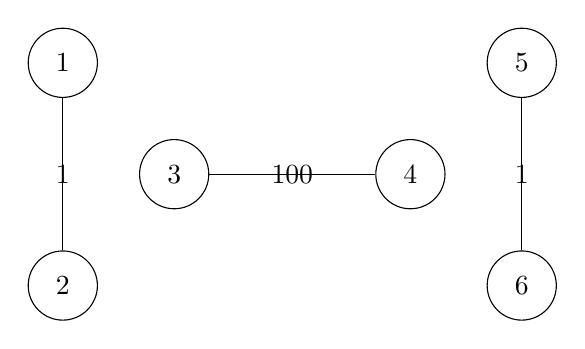
\begin{tikzpicture}[node distance=2cm]
\node[state] (1) {1};
\node[state] (3) [below right of=1] {3};
\node[state] (2) [below left of=3] {2};
\node[state] (4) [right of=3,node distance=3cm] {4};
\node[state] (5) [above right of=4]{5};
\node[state] (6) [below right of=4]{6};
\path[-] (1) edge node{1} (2) (3) edge node{100} (4) (5) edge node{1} (6);
\end{tikzpicture}
\end{figure}
which has cost $102$.

Now, Suppose we make a LP relaxation, it's fairly obvious that we can construct a solution of cost $3$
\begin{figure}[H]
\centering
\caption{LP Relaxation ``Matching''}
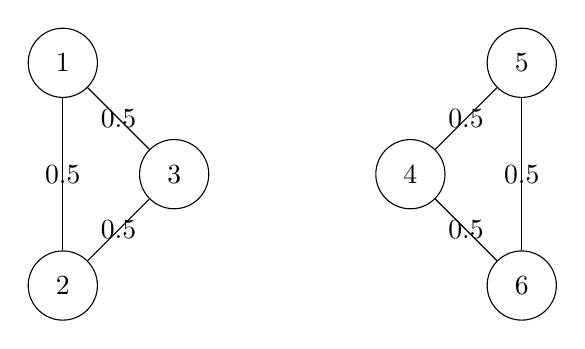
\begin{tikzpicture}[node distance=2cm]
\node[state] (1) {1};
\node[state] (3) [below right of=1] {3};
\node[state] (2) [below left of=3] {2};
\node[state] (4) [right of=3,node distance=3cm] {4};
\node[state] (5) [above right of=4]{5};
\node[state] (6) [below right of=4]{6};
\path[-] (1) edge node{0.5} (2) (1) edge node{0.5} (3) (2) edge node{0.5} (3) (5) edge node{0.5} (6) (5) edge node{0.5} (4) (4) edge node{0.5} (6);
\end{tikzpicture}
\end{figure}
Of course, the answer is no longer integral, and it's impossible to construct an integral solution of the same optimal value; however, the integrality principle formulated above doesn't apply here because the $G$ contains two simple cycles, and hence cannot be bipartite.

Furthermore, we can show that the above solution is optimal by reducing the dimension of the optimization problem. Consider exclusively the constraints given above under LP relaxation, which amounts to 6 equality in addition to restricting the variables to be positive.
\begin{align*}
x_{12} + x_{13} &= 1 \\
x_{12} + x_{23} &= 1 \\
x_{13} + x_{23} &= 1 - x_{34} \\
x_{46} + x_{45} &= 1 - x_{34} \\
x_{56} + x_{45} &= 1 \\
x_{56} + x_{46} &= 1
\end{align*}
This is a system of 6 equations on 7 unknowns, an under-determined system. But, we can reparameterize the system on the value of $x_{34}$ to get a solvable linear system. Letting $\alpha = x_{34}$, we have
$$
\underbrace{\mat{1 & 1 \\ 1& & 1 \\ &1&1 \\ &&&1&1 \\ &&&1&1 \\ &&&&1&1}}_{A}x = e - \alpha e_3 - \alpha e_4
$$
$A$ is invertible, and easily so owing to its nice structure. Let $\mathcal{E}_3$ be the reverse permutation matrix
$$
\mathcal{E}_3 = \mat{&&1\\&1\\1}
$$
then the solution to the above system is just
$$
x = \pa{A - \mat{\mathcal{E}_3 \\ & \mathcal{E}_3}}\pa{e - \alpha e_3 - \alpha e_4}
$$
which admits the solution
$$
x = \frac{1}{2}\mat{1 + \alpha \\ 1 - \alpha \\1 - \alpha \\1 - \alpha \\1 - \alpha \\1 + \alpha}
$$
and since the objective function is just $e^Tx + 100\alpha$, we see that we're trying to minimize the one-variable \textbf{linear} system
$$
f(\alpha) = \frac{1}{2}(2 + (1+\alpha) + 4(1-\alpha)) + 100\alpha
$$
given that the objective is linear, its derivative is constant and nonzero, so $\min_\alpha f(\alpha)$ subjected to $x,\alpha > 0$ can only occur at $\alpha = 0$, which gives the solution above (each non $(3,4)$ edge is assigned a value of $\frac{1}{2}$).

\item Let $S$ be a set containing $m$ nodes, where $m$ is odd. For any perfect matching, what can you say about the number of arcs that have one endpoint in $S$ and the other endpoint outside of $S$? Use this to derive a collection of linear inequalities that every integer solution to the original IP satisfies.

\vspace{4mm}
Suppose we partition the vertices $V$ into $S$ and $T = V\backslash S$, then it must be the case that at least one edge in the cut between $S$ and $T$ is in the perfect matching.

Suppose not, then because $S$ is odd, one of its elements cannot possibly be in a match with any other vertices in $S$, but since there are no matchings between $S$ and the rest of $V$, there are no vertices to which that abandoned vertex is matched to. But we've already assumed that we have a perfect match, a contradiction.\hfill\qed

Finally, this gives an additional constraint on which we can work from.

Let $\mathcal{P}_n$ be the collection of n-permutations of the set $\Rec{1,\cdots,n}$ up to set isomorphism. We should add in the additional constraint that
$$
\forall p \in \mathcal{P}_{2n+1}(v). \sum_{i \in p, j \notin p, (i,j) \in E} x_{ij} \ge 1
$$
(note that we cannot provide a useful upper bound here)

\item Use the same type of an inequality that you derived in the previous part to strengthen
the LP relaxation in part (iii), in the sense that once you add this constraint to the formulation, the optimal LP solution you found in (iii) would no longer be feasible for the new LP
relaxation.

\vspace{4mm}
We can just drop in the same exact collection of constraints
$$
\forall p \in \mathcal{P}_{2n+1}(v). \sum_{i \in p, j \notin p,(i,j) \in E} x_{ij} \ge 1
$$
The LP relaxation solution found above is now rejected because for the 3-permutation corresponding to partial identity, we have the constraint that, letting $p = \Rec{1,2,3}$, then
$$
\sum_{i \in p, j \notin p, (i,j) \in E} x_{ij} = x_{34} \ge 1
$$
which is can't be satisfied as we've assigned $x_{34} = 0$.
\end{enumerate}
\end{enumerate}

\end{enumerate}

\end{document}
